\chapter{Kommunikationsmodule}
\label{chap:Kommunikationsmodule}
Gemäss Auftraggeber sollen Daten der Wetterstation per SMS abrufbar und der Standort der Wetterstation ermittelbar sein. Um SMS empfangen und auch senden zu können, wird ein GSM-Modul benötigt. Weiter wird ein GPS-Modul benötigt, um eine Standortermittlung durchführen zu können. Der SIM808 ist ein Kombinationsmodul aus GSM und GPS, was nicht nur Platz auf dem PCB, sondern auch Energietechnisch und Preislich Vorteile bietet, da nur ein Modul betrieben werden muss. Aus diesen Gründen wurde der SIM808 implementiert.

\section{SIM808}
{\begin{minipage}[b][6cm][t]{0.52\textwidth}
Der SIM808 (Abbildung \ref{fig:SIM808}) verfügt über GSM/GPRS (Global System for Mobile Communications / General Packet Radio Service), GPS (Global Positioning System) und BT (Bluetooth). Für die Wetterstation wird das GSM und das GPS verwendet. Tabelle \ref{tab:SIM808} zeigt die elektrischen Spezifikationen des SIM808. \cite{SIM808}\\
\end{minipage}}
{\begin{minipage}[b][6cm][t]{0.47\textwidth}
\centering
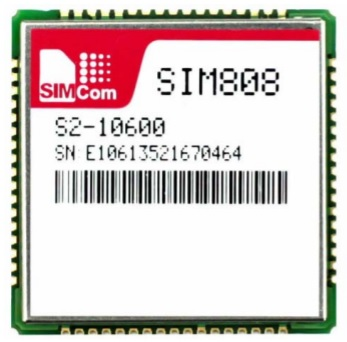
\includegraphics[width=0.7\textwidth]{graphics/SIM808/SIM808.JPG}
\captionof{figure}{SIM808 von Vorne 
\cite{SIM808}}
\label{fig:SIM808}
\end{minipage}}


\begin{table}[h]
\centering
  \caption{Elektrische Spezifikationen des SIM808 \cite{SIM808}}
\begin{tabular}{lllll}
\toprule 
\textbf{Parameter} & \textbf{Min} & \textbf{Typ} & \textbf{Max} & \textbf{Einheit} \\ 
\midrule 
Power Supply & 3.4 &  & 4.4 & V \\ 
Power saving &  & 1 &  & mA \\ 
Transmitting power (GSM) &  & 2 &  & W \\ 
SIM interface support &  & 1.8/3 &  & V \\ 
Power consumption (Idle GSM) &  & 22.1 &  & mA \\
Power consumption (Data GSM) &  & 445.82 &  & mA \\
Power consumption (TX Burst GSM) &  &  & 2 & A \\
Power consumption (GPS Acquisition) &  & 42 &  & mA \\ 
Power consumption (GPS Continuous tracking) &  & 24 &  & mA \\ 
\bottomrule
\end{tabular} 
\label{tab:SIM808} 
\end{table}

Damit das GSM über den SIM808 genutzt werden kann, wird eine SIM-Karte benötigt. Dafür wurde eine Prepaid M-Budget SIM-Karte von Andres Minder erworben, welche jedoch Vertragsbedingt persönlich ist und nicht Teil der Wetterstation bleibt. Diese SIM-Karte wird lediglich zu Testzwecken genutzt und muss später durch eine SIM-Karte des Endbenutzers ersetzt werden. Die SIM-Karte wird mit einem SIM-Karten-Adapter (Speicherkartensteckverbinder) auf dem PCB integriert und mit dem SIM808 verbunden.\\
